\section{Implementacja}
W niniejszym rozdziale opisano szczegółowo implementację komponentów składających się na budowę emulatora: pamięć, procesor, wybranych instrukcji maszyny wirtualnej, deasembler, urządzenia wejścia i wyjścia, a także moduł obsługujący argumenty wiersza poleceń i główną pętlę programu.

\subsection{Moduł pamięci}
Pamięć maszyny wirtualnej została zaimplementowana jako oddzielna klasa, której zadaniem jest stworzenie \emph{tablicy bitowej} (ang.\emph{bytearray}) mającej rozmiar odpowiadający wielkości pamięci \textit{RAM} ze specyfikacji CHIP-8 (4096B) \cite{Cowgod}. Następnie od zerowego indeksu wczytywany jest do niej zestaw czcionek. Są one zapisane w tablicy jako cyfry szesnastkowe. 

\begin{figure}[!htb]
	\begin{center}
		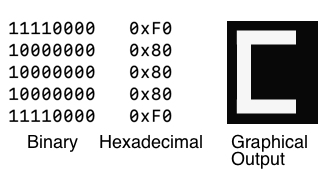
\includegraphics[scale=0.6]{images/c8_fonts_repr}
		\caption{Konwersja litery "C" z liczby binarnej do szesnastkowej i postaci graficznej}
	\end{center}
\end{figure}

Kolejną metodą klasy \textit{Memory} jest ta, odpowiedzialna za wczytanie pliku binarnego z programem. Działa ona podobnie do poprzednio przedstawionej funkcji, odpowiedzialnej za wczytywanie czcionek, z tą różnicą, że wykorzystana została wbudowana w język Python funkcja \textit{open()} z argumentem  \textit{'rb'} (\textit{read binary}), odpowiedzialnym za wczytywanie pliku w postaci binarnej. Tym razem dane są wczytywane do pamięci \textit{RAM} od adresu z indeksem 512, czyli przestrzeni specjalnie przeznaczonej na zewnętrzny program \cite{Cowgod}.

\subsection{Deasembler}
Deasembler to dodatkowy moduł zaimplementowany w celu lepszego zapoznania się z instrukcjami procesora. Podobnie jak kod odpowiedzialny za emulowanie procesora. Wczytuje on instancje klasy odpowiedzialnej za zarządzanie pamięcią, a następnie za pomocą metody \textit{get\_opcode}, przekazuje wartość do zmiennej \textit{opcode}. Następnie wydobywane są argumenty instrukcji, czyli bajty, który nie służą do rozpoznania wykonywanej operacji. Wskazują one jedynie odpowiednie numery rejestrów lub bajty które zostaną do nich dodane, a następnie przekazuje je do atrybutu \textit{args}. Kolejnym krokiem jest zamaskowanie argumentów w zmiennej trzymającej kod instrukcji, tak, aby posiadała ona informacje odpowiadające jedynie za identyfikacje kodu procesora. Otrzymane dane służą jako klucz w słowniku, jego wartością jest natomiast funkcja zwracająca podstać mnemoniczną danego \textit{słowa}. Na końcu wszystkie otrzymane informacje są odpowiednio formatowane jako zmienna typu \textit{string}. Cała procedura powtarzana jest w pętli od pierwszego adresu w pamięci do ostatniego, a licznik programu za każdą iteracją jest inkrementowany o 2.
\begin{figure}[!htb]
	\begin{center}
		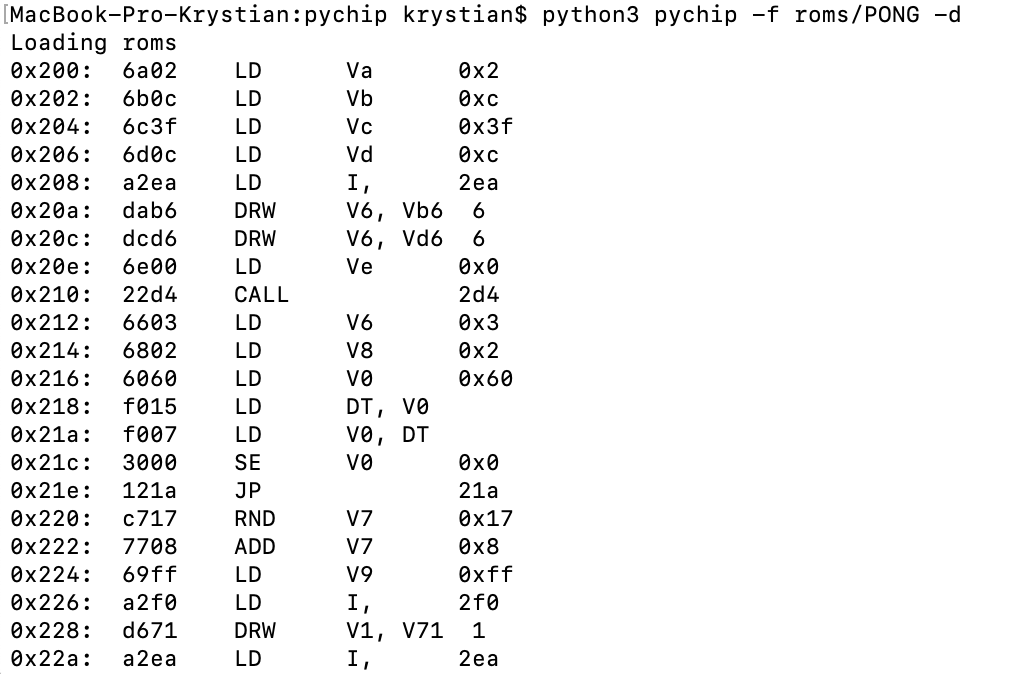
\includegraphics[scale=0.6]{images/outputDasm.png}
		\caption{Efekt działania modułu deasemblera}
	\end{center}
\end{figure}

\subsection{Moduł procesora}
Klasa \textit{Processor} przyjmuje instancje pamięci jako argument, następnie przy inicjalizacji tworzony jest słownik trzymający stan rejestrów \textit{V}, \textit{S} i \textit{I}, a także \textit{delay} i \textit{sound}. Następnie tworzone są zmienne, wskazujące na komórkę w pamięci \textit{RAM}, czyli \textit{program counter} i wskaźnik na stos \textit{stack pointer}. Kolejnymi polami są: lista odzwierciedlająca bufor ekranu i zmienna typu \textit{true/false} trzymająca informacje, czy zawartość ekranu była edytowana. Jest ona używana do sprawdzenia, czy moduł odpowiedzialny za wyświetlanie obrazu potrzebuje wygenerować na nowo grafikę. Ostatnimi atrybutami są tworzone przy inicjalizacji: \textit{pressed\_key} posiadający ostatniego klikniętego klawisza i słownik \textit{instructions}.\\

Działanie klasy procesora oparte jest o wczytywanie obecnie wskazanej przez \textit{program counter} i następnej komórki do specjalnej zmiennej nazwanej \textit{operand}. Spowodowane jest to tym, że kody procesora mają postać szesnastobitową, a pamięć jest ośmiobitowa. Z tego względu wartość \textit{operand} musi zostać przesunięta o 8 bitów w prawo, przez co do tej zmiennej dołączane jest osiem zer, następnie wykorzystuje operacje alternatywy, dzięki temu wartość z obu komórek włączana jest do zmiennej \textit{operand}. \\

Wszystkie instrukcje procesora są zaimplementowane jako funkcje. W Pythonie sama funkcja bez jej wywołania jest traktowana jako obiekt, dlatego można go wykorzystać jako wartość w słowniku, którego kluczami będą liczby od 0x0 do 0xF, odpowiadają one zakresowi starszych półbajtów pierwszych bitów instrukcji przedstawionych w \textit{Cowgod's CHIP-8 Technical Reference} \cite{Cowgod}.

\begin{lstlisting}[caption={Budowa słownika \textit{instructions}},captionpos=b]
self.instructions = {
    0x1: self.jp_addr,
    0x2: self.call_addr,
    0x3: self.se_vx_byte,
    0x4: self.sn_vx_byte,
    0x5: self.se_vx_vy,
    0x6: self.ld_vx_byte,
    0x7: self.add_vx_byte,
    0x9: self.sne_vx_vy,
    0xa: self.ld_i_addr,
    0xc: self.rnd_vx_byte,
    0xd: self.drw_vx_vy_n,
    0x0: self.sys_ops,
    0x8: self.logical_ops,
    0xf: self.rest_ops,
    0xE: self.press_ops
}
\end{lstlisting}

Po dostarczeniu wartości pamięci do zmiennej \textit{operand} wybierany jest z niej starszy półbajt pierwszego bajta, który staje się kluczem do wcześniej wspomnianego słownika \textit{instructions}. Na jego podstawie wybierana zostaje instrukcja, która będzie wykonywana. W razie gdyby taki klucz nie istniał, wykonywana jest pusta funkcja lambda, która wyświetli informacje o błędzie. Zanim to jednak się stanie, wartość licznika programu podnoszona\footnote{Wartość licznika programu inkrementowana jest za każdym razem o 2, tak aby pominąć wykorzystane już komórki, które pełnią role młodszych bajtów w zmiennej \textit{operand}} jest o 2. 

\begin{lstlisting}[caption={Framgent kodu, służący do wywoływania instrukcji procesora.},captionpos=b]
def get_operand(self):
    return self.memory[self.pc] << 8 | self.memory[self.pc + 1]

def extract_opcode(self):
    return (self.operand & 0xf000) >> 12

def execute_instruction(self):
    self.operand = self.get_operand()
    opcode = self.extract_opcode()
    self.pc += 2
    self.instructions.get(opcode, lambda x: ...)()
\end{lstlisting}

Po wykonaniu kodu operacyjnego zostaje zmieniana jeszcze wartość zegarów emulowanego urządzenia.
\subsubsection{Instrukcje}
Istnieją przypadki, gdzie pod wspomnianym wcześniej identyfikatorem można wyróżnić kilka kodów procesora, wówczas są one weryfikowane na podstawie pozostałych bitów wewnątrz jednej funkcji za pomocą instrukcji warunkowej \textit{if}. Takimi przypadkami są klucze w słowniku o wartościach: \textit{0x0}, \textit{0x8}, \textit{0xE}, \textit{0xF}.

Implementacja poszczególnych z ich wygląda następująco:

\begin{itemize}
  \item Wywołaj adres z stosu (\textit{call\_addr}):
\end{itemize}
Do rejestru \textit{S}, dodawana jest wartość \textit{licznika programu}, a \textit{wskaźnik stosu} jest inkrementowany o jeden. Następnie za pomocą operacji binarnej \textit{AND}, z wartości \textit{operand} wybieranych jest 12 ostatnich bitów. Zostają one przypisane do \textit{licznika programu}.
\begin{lstlisting}[caption={Framgent kodu, odpowiedzialny za instrukcje \textit{call\_addr}},captionpos=b]
self.registers['s'].append(self.pc)
self.sp += 1
self.pc = self.operand & 0x0fff
\end{lstlisting}

\begin{itemize}
  \item Pomiń następną instrukcje jeżeli \textit{Vx==Vy} (\textit{sne\_vx\_vy}):
\end{itemize}
Dzięki operacji binarnej \textit{AND} z pierwszego bajta \textit{słowa} wyciągane są młodsze bity. W celu usunięcia drugiego bajta wykonywane jest przesunięcie bitowe o 8. Uzyskana zmienna posłuży do identyfikacji rejestru \textit{Vx}. Następnie w podobny sposób ze \textit{słowa} wyciągana jest wartość do identyfikacji rejestru \textit{Vy}. Jeżeli wartości z rejestrów \textit{Vx} i V{y} są sobie równe, to \textit{licznik programu} inkrementowany jest o 2.
\begin{lstlisting}[caption={Implementacja instrukcji \textit{sne\_vx\_vy}},captionpos=b]
x = (self.operand & 0x0f00) >> 8
y = (self.operand & 0x00f0) >> 4
if self.registers['v'][x] == self.registers['v'][y]:
    self.pc += 2
\end{lstlisting}

\begin{itemize}
  \item Dodaj \textit{Vx} do \textit{Vy} (\textit{add\_vx\_vy}):
\end{itemize}
Wartość z rejestru \textit{Vy} jest dodawana do rejestru \textit{Vx}. Jeżeli po dodaniu \textit{Vx} przekracza 256 bitów, ustawiana jest flaga w rejestrze \textit{Vf}. Sprawdzona zmienna za pomocą instrucji \textit{AND} zostaje zredukowana do wartości mniejszej niż 256. W przeciwnym przypadku, flaga \textit{Vf} zostaje wyzerowana.
\begin{lstlisting}[caption={Implementacja instrukcji \textit{add\_vx\_vy}},captionpos=b]
self.registers['v'][x] += self.registers['v'][y]
if self.registers['v'][x] > 0xFF:
    self.registers['v'][0xF] = 1
    self.registers['v'][x] &= 0xFF
else:
	self.registers['v'][0xF] = 0
\end{lstlisting}


\newpage

\subsection{Moduł wejścia/wyjścia}
Podstawą tego modułu jest klasa \textit{Window}, dziedzicząca z\textit{tkinter.Tk}. Odpowiada ona za podstawę interfejsu użytkownika wyświetlającego emulacje, jego konfiguracje, a także pasek menu przy górnej belce. Przy jej inicjalizacji zostaje ustalony rozmiar okna, a także zablokowana możliwość ręcznego zmieniania jego wielkości. Następnie zostaje ustalona kolejność komend na pasku narzędzi. Pierwszą opcją jest \textit{file}, w której zawiera funkcja \textit{open}. Odpowiedzialną za wywołanie okna wyboru pliku. Jest to standardowy \textit{dialog} z pakiety \textit{tkinter.filedialog} \cite{TKINTER}.

\begin{figure*}[!htb]
\begin{center}
	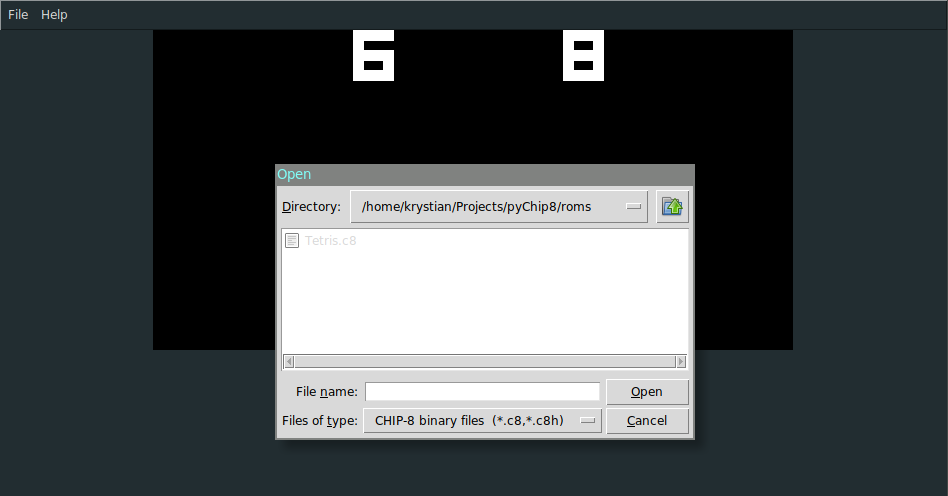
\includegraphics[scale=0.32]{images/fileDialog}
	\caption{Dialog do wybierania plików (system \textit{GNU/Linux })}
\end{center}
\end{figure*}

 W opisywanym projekcie potrzebne były różne konfiguracje dla każdej ze wspieranych platform. Dla przykładu system windows do przedstawienia ścieżek używa znaku \textit{lewego ukośnika}, gdy w platformach \textit{uniksowych} jest to zwykły ukośnik. Dodatkowo \textit{dialog} w systemie\textit{macOS}  wyświetlający pliki nie posiada możliwości wyboru formatu, więc w tym przypadku, trzeba było pozostawić opcję wyboru tylko wszystkich plików.
 
\begin{figure*}[!htb]
\begin{center}
	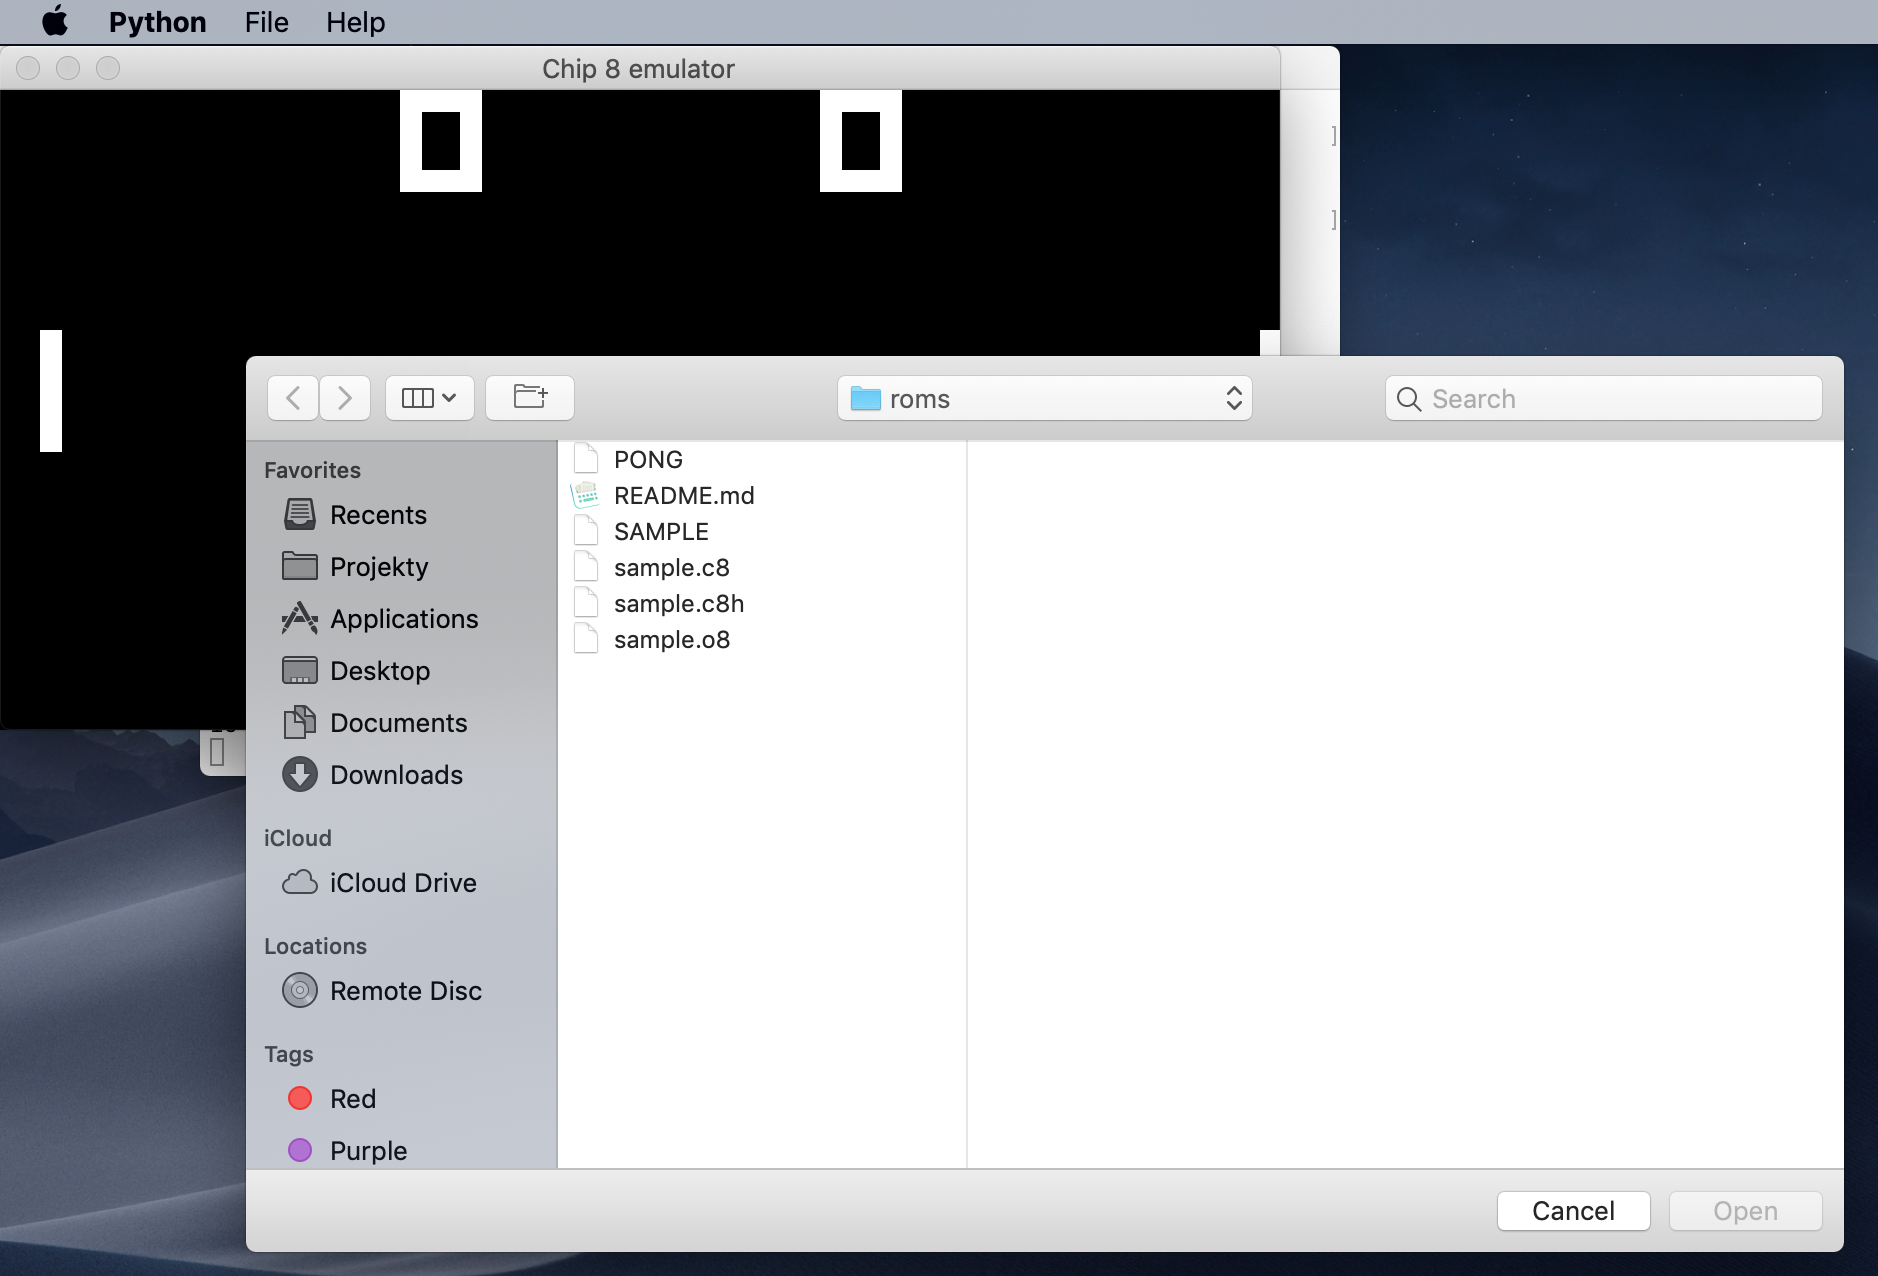
\includegraphics[scale=0.3]{images/fileDialog-macos}
	\caption{Dialog do wybierania plików (system \textit{macOS})}
\end{center}
\end{figure*}

\newpage

Kolejną opcją jest \textit{reset}, gdzie przywracane są wszystkie rejestry do wartości początkowych, a emulacja rozpoczyna się na nowo. Następną sekcją jest \textit{help}, która zawiera opcje \textit{about}, w których są zawarte informacje o wersji programu z linkiem do \textit{githuba} projektu i \textit{changelog}, gdzie opisano zmiany w wersja. We wszystkich tych przypadkach skorzystano z modułu \textit{tkinter.messagebox} \cite{TKINTER}, który wyświetla okienka informacyjne. System \textit{macOS} posiada pasek menu, który zmienia się zależnie od aplikacji przez co, nie ma pojawia się pasek narzędzi w okienku aplikacji. Ma on dodatkową sekcje, która ma taką samą nazwę jak ta aplikacji. Z tego względu dla tej platformy dodano funkcję, która zmienia wyświetlane w nim informacje na te z sekcji \textit{about}.


\begin{figure*}[!htb]
\begin{center}
	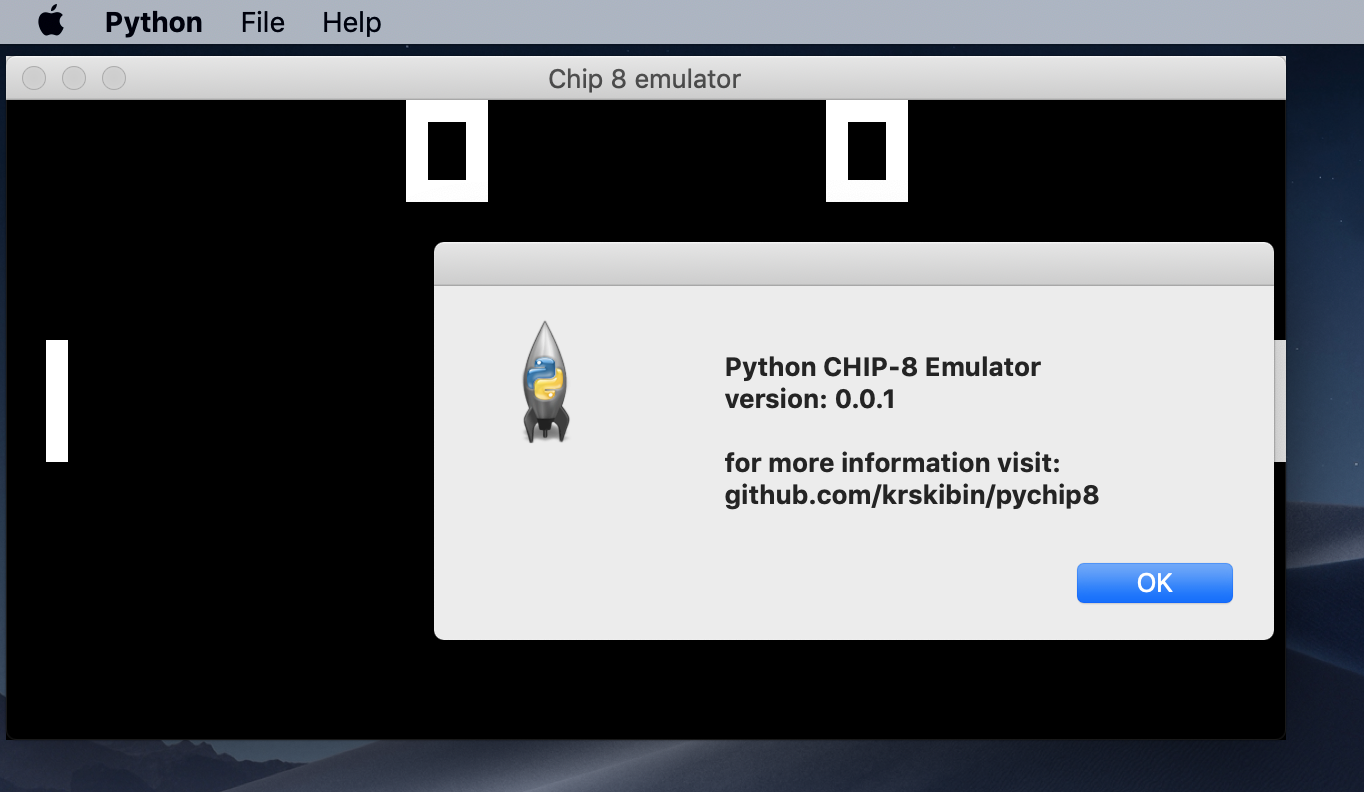
\includegraphics[scale=0.4]{images/aboutSection}
	\caption{\textit{Messagebox} z informacjami (system macOS)}
\end{center}
\end{figure*}

Następnym zaimplementowanym fragmentem kodu jest klasa \textit{Screen}. Odpowiada ona za sterownie wcześniej opisaną klasę \textit{Window}. To przy jej inicjalizacji podpinane są zdarzenia dla kliknięcia klawisza. Są to funkcje:\textit{key\_down} i \textit{key\_up}. Ich zadaniem jest mapowanie klawiszy z klawiatury użytkownika na heksadecymalną, którą oryginalnie obsługiwały komputery dla których był napisany CHIP-8 \cite{COSMAC}.

\begin{lstlisting}[caption={Słownik z mapowaniem klawiszy (wartości w nawiasach, to rzeczywiste klawisze)},captionpos=b]
self.keymap = {
   '1': 1, '2': 2, '3': 3, '4': 12, 'q': 4, 'w': 5,
   'e': 6, 'r': 13, 'a': 7, 's': 8, 'd': 9, 'f': 14,
   'z': 10, 'x': 0, 'c': 11, 'v': 15,
}
\end{lstlisting}
Do tej klasy podpięto również obiekt \textit{tkinter.Canvas} \cite{TKINTER}, który dostarcza interfejs pozwalający na rysowanie kształtów. Wykorzystuje ją metoda  \textit{draw\_pixel}, której zadaniem jest iteracja po \textit{buferze} z modułu procesora i gdy napotka wartość \textit{1}, to w tym miejscu, na odpowiednie przeskalowanym kanwasie rysuje kwadrat. Dla oszczędzenia pamięci, przed wywałniem tej metody, wszystkie obiekty z kanwasu są usuwane. Ostatnią metodą w tym module jest ta odpowiedzialna za czyszczenie ekranu emulatora. Jest ona interfejsem do metody zaimplementowanej w \textit{tkinter} i przyjmuje ona specjalną stałą \textit{tkinter.ALL} zawierającą referencje do każdego obiektu kanwasu.


\subsection{Główny moduł programu}

Jest to moduł odpowiedzialny za ciągłe działanie emulatora. Tworzone są w nim instancje zaimplementowanych klas, a także przekazane wymagane argumenty. Następnie ustalana jest rozdzielczość ekranu, obecność dźwięku i szybkość działania procesora. Kolejnym krokiem jest rozpoczęcie \textit{głównej pętli aplikacji}, która z każdą iteracją wykonuje kolejną instrukcje procesora, a także definiuje jego prędkość taktowania.
\begin{figure*}[!htb]
\begin{center}
	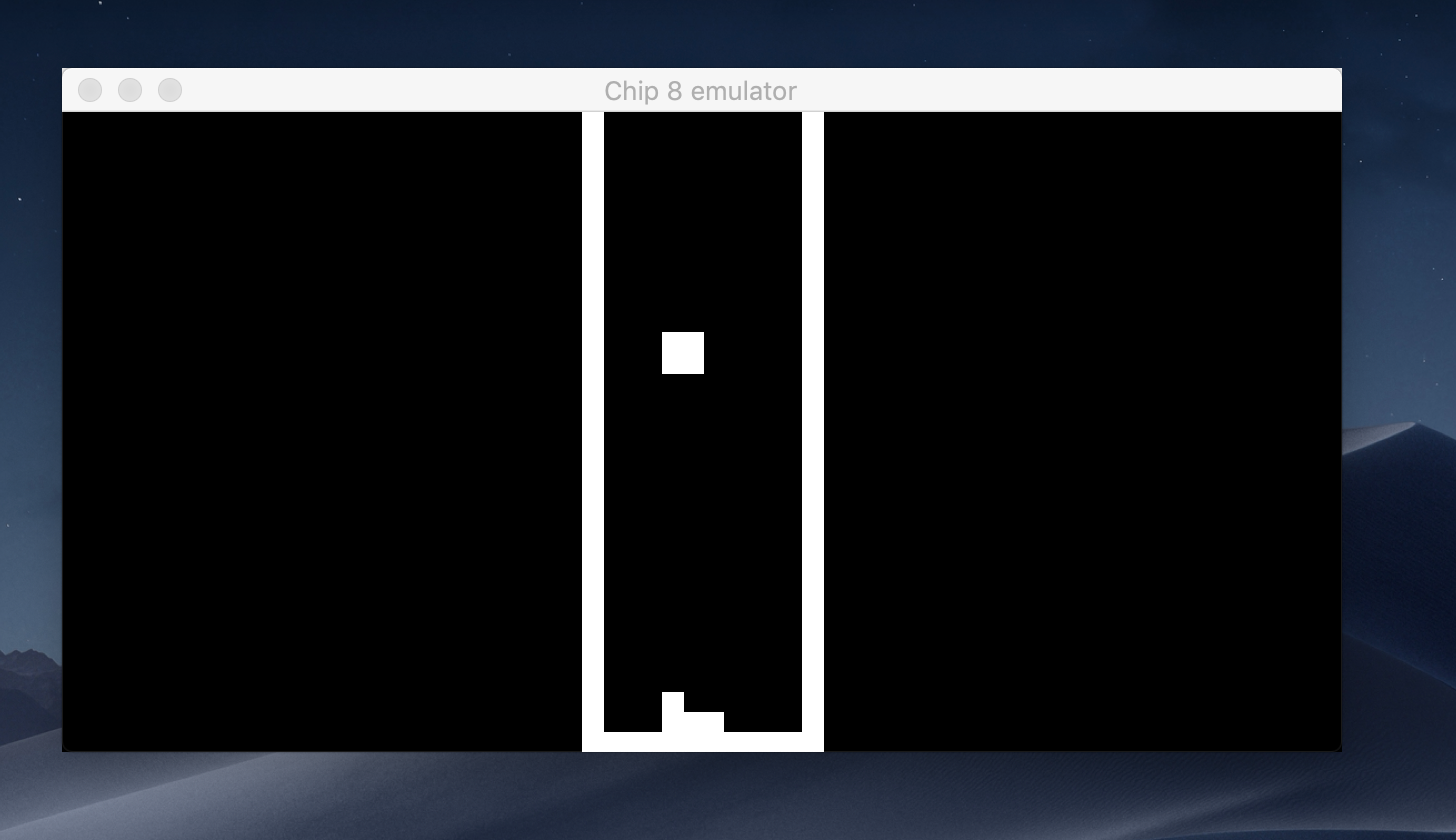
\includegraphics[scale=0.4]{images/workingApp}
	\caption{Działający emulator, gra \textit{TETRIS} (autor Fran Dachille, rok 1991)}
\end{center}
\end{figure*}

W module znajduje się również implementacja interfejsu linii poleceń. Jest to obiekt z pakietu \textit{argparse}, który za pomocą metody \textit{add\_argument} \cite{Argparse}, definiuje opcje, przyjmowane przez program przy wywołaniu, a także ich opis, typ i nazwy zmiennych do których zostaną przepisane  one w kodzie aplikacji.

\begin{lstlisting}[caption={Wynik uruchomienia programu z opcją \textit{-h}},captionpos=b]
$../pychip: python pychip -h
usage: [-h] [-f ROMS] [-d] [-r RES] [-t DLY]

Chip8 emulator

optional arguments:
  -h, --help            show this help message and exit
  -f ROMS, --file ROMS  use to provide roms file
  -d, --disassembler    run disassembler for given roms file
  -r RES, --res RES     set CHIP-8 screen resolution
  -t DLY, --time DLY    set emulation delay time

\end{lstlisting}






